\section{Problém obchodního cestujícího}

Problém obchodního cestujícího budeme zkracovat na TSP, z anglického názvu
Travelling salesman problem. Úkolem je najít nejkratší cestu, která navštíví
všechny města a vrátí se zpět do prvního, za předpokladu, že mezi každými dvěma
městy vede silnice. V řeči teorie grafů můžeme problém definovat následovně.

\medskip
\noindent\textbf{Optimalizační verze:} V daném ohodnoceném úplném grafu najděte
nejkratší Hamiltonovskou kružnici.

\noindent\textbf{Rozhodovací verze:} Existuje v daném ohodnoceném úplném grafu
Hamiltonovská kružnice kratší než $k$?
\medskip

Obecně nemusí platit trojúhelníková nerovnost, ale předpokládáme, že váhy
jednotlivých hran jsou nezáporné.

\subsection{Obtížnost TSP}

\vt TSP je $\NP$-úplný.

\dk Převodem na Hamiltonovskou kružnici v grafu $G = (V,E)$. Hranám úplného
grafu, které jsou v $E$ přiřadíme váhu 1, hranám které nejsou v $E$ váhu 2 a
ptáme se, zda existuje řešení TSP s váhou $|V|$. TSP $\in \NP$ dokážeme tak, že
použijeme výsledné pořadí vrcholů jako certifikát.\footnote{Řešíme rozhodovací
verzi, takže stačí ověřit, že je to kružnice s délkou nejvýše $k$ -- nemusíme
ověřovat, že je nejkratší, to by samozřejmě bylo těžší.}

Z toho, že TSP je $\NP$-úplný je jasné, že neznáme žádný polynomiální
deterministický algoritmus, který by TSP řešil. Známe ale několik aproximačních
algoritmů, které najdou přijatelně dobré (i když ne nejlepší) řešení.

\subsection{Aproximační algoritmy na TSP}

Všechny aproximační algoritmy pro TSP předpokládají, že platí trojúhelníková
nerovnost.

\begin{wrapfigure}{R}{4.5cm}
\centering
\vspace{-0.4cm}
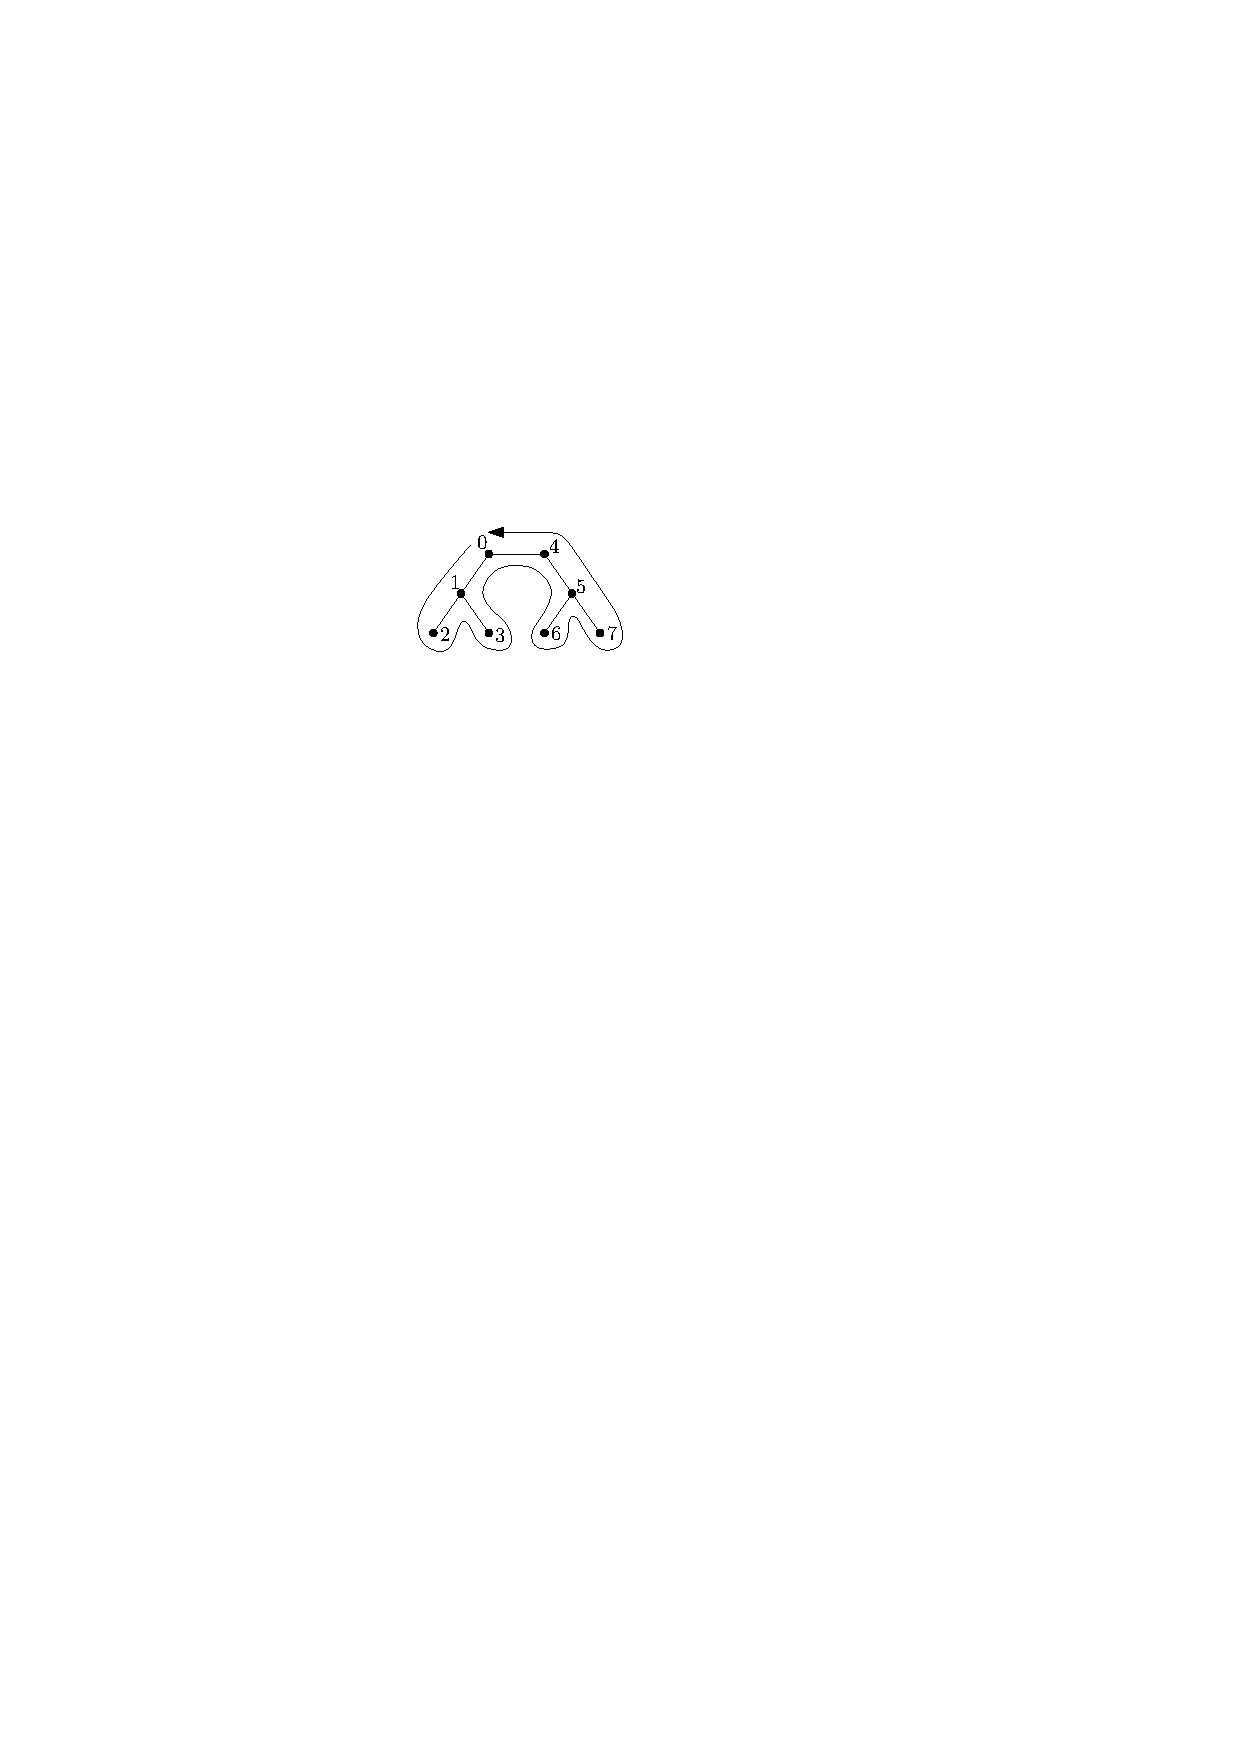
\includegraphics[width=4.5cm]{img/tsp-aproximace.pdf}
\end{wrapfigure}

\alg (Aproximace přes kostry) Nejprve najdeme minimální kostru grafu $G$. Ta je
dolním odhadem na řešení TSP.\footnote{Kdyby bylo řešení TSP menší, než
minimální kostra, pak bychom dostali menší kostru vypuštěním libovolné hrany z
řešení TSP.} Začneme z libovolného vrcholu a určíme pořadí vrcholů tak, že
půjdeme okolo rovinného nakreslení minimální kostry po směru hodinových ručiček.
Toto pořadí vrcholů vydáme jako výsledek.

\vt Aproximace přes kostry je polynomiální 2-aproximační algoritmus pro TSP s
trojúhelníkovou nerovností.

\alg (Christofides)
\begin{enumerate*}
\item Nalezneme minimální kostru $T$ grafu $G$.
\item Označme $O$ vrcholy s lichým stupněm v $T$. Nalezneme perfektní párování
$M$ na vrcholech $O$ s minimální váhou.
\item Sjednotíme $T$ a $M$ a získáme multigraf $H$.
\item Najdeme Eulerovský tah v $H$ ($H$ je souvislý a má stupně všech vrcholů sudé).
\item Vytvoříme Hamiltonovskou kružnici tak, že půjdeme po Eulerovském tahu a
budeme přeskakovat již navštívené vrcholy.
\end{enumerate*}

\vt Christofides je polynomiální $3\over 2$-aproximační algoritmus pro TSP s
trojúhelníkovou nerovností.

\dk Všimněme si nejprve, že přeskakováním již navštívených vrcholů nikdy
nedostaneme delší cestu, což plyne z trojúhelníkové nerovnosti.

Označme $A$ množinu hran, která je optimálním řešením TSP v úplném grafu $G =
(V,w)$. Protože graf $(V,A)$ je souvislý, obsahuje nějakou kostru $T$ a zjevně
$w(A) \ge w(T)$. Označme $B$ množinu hran, která je optimálním řešením TSP v
úplném grafu $(O,w)$. Protože platí trojúhelníková nerovnost, musí být $w(A) \ge
w(B)$.

Ukážeme, že existuje perfektní párování na $O$, které váží méně než $w(B)/2 \le
w(A)/2$. $O$ jistě obsahuje sudý počet vrcholů, tedy existuje maximální
párování. Vezmeme graf $(O,B)$, který sestává právě z jedné Hamiltonovské
kružnice. V této kružnici vezmeme buď všechny liché hrany, nebo všechny sudé
hrany a prohlásíme je za párování. Protože váha celé kružnice je $w(B)$, pak
váha lichých nebo sudých hran musí být nejvýš $w(B)/2$. Tedy, $w(M) + w(T) \le
w(A) + w(A)/2$ a algoritmus je $3\over 2$-aproximační.
\qed

